% !TEX root = ../main.tex
\section{Learning to Reweight Examples}

In this section, we derive our model from a meta-learning objective towards an online approximation
that can fit into any regular supervised training. We give a practical implementation suitable for
any deep network type and  provide theoretical guarantees under mild conditions that our algorithm
has a convergence rate of $O(1/\epsilon^2)$. Note that  this is the same as that of stochastic
gradient descent (SGD).

\subsection{From a meta-learning objective to an online approximation}

Let $(x,y)$ be an input-target pair, and $\{(x_i, y_i), 1 \le i \le N\}$ be the training set. We
assume that there is a small unbiased and clean validation set $\{(x^v_i, y^v_i), 1 \le i \le M\}$,
and $M \ll N$. Hereafter, we will use superscript $v$ to denote validation set and subscript $i$ to
denote the $i^{th}$ data. We also assume that the training set contains the validation set;
otherwise, we can always add this small validation set into the training set and leverage more
information during training.

Let $\Phi (x,\theta)$ be our neural network model, and $\theta$ be the model parameters. We consider
a loss function $C(\hat{y}, y)$ to minimize during training, where $\hat{y} = \Phi (x, \theta)$.

In standard training, we aim to minimize the expected loss for the training set: $\frac{1}{N}
\sum_{i=1}^N C(\hat{y}_i, y_i)=\frac{1}{N} \sum_{i=1}^N f_i(\theta)$, where each input example is
weighted equally, and $f_i(\theta)$ stands for the loss function associating with data $x_i$. Here
we aim to learn a reweighting of the inputs, where we minimize a weighted loss:
\begin{equation}
\label{eq:theta_star}
\theta^*(w) = \argmin_\theta \sum_{i=1}^N w_i f_i(\theta),
\end{equation}
with $w_i$  unknown upon beginning. Note that $\{w_i\}_{i=1}^N$ can be understood as  training
hyperparameters, and the optimal selection of $w$ is based on its validation performance:
\begin{equation}\label{eq:w_star}
w^* = \argmin_{w, w \ge 0} \frac{1}{M} \sum_{i=1}^M f_i^v(\theta^*(w)).
\end{equation}
It is necessary that $w_i \ge 0$ for all $i$, since  minimizing the negative training loss can
usually result in unstable behavior.

\paragraph{Online approximation} Calculating the optimal $w_i$ requires two nested loops of
optimization, and every single loop can be very expensive. The motivation of our approach is to adapt
online $w$ through a single optimization loop. For each training iteration, we inspect the descent
direction of some training examples locally on the training loss surface and reweight them
according to their similarity to the descent direction of the validation loss surface.

For most training of deep neural networks, SGD or its variants are used to  optimize such loss
functions. At every step $t$ of training, a mini-batch of training examples $\{(x_i, y_i), 1 \le i
\le n\}$ is sampled, where $n$ is the mini-batch size, $n \ll N$. Then the parameters are adjusted
according  to the descent direction of the expected loss on the mini-batch. Let's consider vanilla
SGD:
\begin{align}
\theta_{t+1} = \theta_t - \alpha \nabla \left( \frac{1}{n}\sum_{i=1}^n f_i(\theta_t) \right),
\end{align}
where $\alpha$ is the step size.

We want to understand what would be the impact of training example $i$ towards  the performance of
the validation set at training step $t$. Following a similar analysis to \citet{kohL17influence}, we
consider perturbing the weighting by $\epsilon_i$ for each training example in the mini- batch,
\begin{align}
f_{i,\epsilon}(\theta) &= \epsilon_i f_i(\theta),\\
\hat{\theta}_{t+1}(\epsilon) &= \theta_t - \alpha \nabla \sum_{i=1}^n
\left. f_{i,\epsilon}(\theta) \right\vert_{\theta=\theta_t}.
\end{align}
We can then look for the optimal $\epsilon^*$ that minimizes the validation loss $f^v$ locally at step $t$:
\begin{align}
\epsilon^*_t = \argmin_\epsilon \frac{1}{M} \sum_{i=1}^M f^v_i(\theta_{t+1}(\epsilon)).
\end{align}
Unfortunately,  this can still be quite time-consuming. To get a cheap estimate of $w_i$ at step
$t$, we take a single gradient descent step on a mini-batch of validation samples wrt.
$\epsilon_t$, and then rectify the output to get a non-negative weighting:
\begin{align}
\label{eq:meta-gradient}
u_{i,t} &= -\eta \frac{\partial}{\partial \epsilon_{i,t}} \frac{1}{m} 
            \sum_{j=1}^m \left. f_j^v(\theta_{t+1}(\epsilon)) \right \vert_{\epsilon_{i,t}=0},\\
\tilde{w}_{i,t} &= \max(u_{i,t}, 0).
\end{align}
where $\eta$ is the descent step size on $\epsilon$.

To match the original training step size, in practice, we can consider normalizing the weights of
all examples in a training batch so that they sum up to one. In other words, we choose to have
a hard constraint within the set $\{w: \lVert w \rVert_1 = 1 \} \cup \{0\}$.
\begin{align}
w_{i,t} = \frac{\tilde{w}_{i, t}}{(\sum_j \tilde{w}_{j, t}) + \delta(\sum_j \tilde{w}_{j, t})},
\end{align}

where $\delta(\cdot)$ is to prevent the degenerate case when all $w_i$'s in a mini-batch are zeros,
i.e. $\delta(a) = 1$ if $a = 0$, and equals to $0$ otherwise. Without the batch-normalization step,
it is possible that the algorithm modifies its effective learning rate of the training progress, and
our one-step look ahead may be too conservative in terms of the choice of learning rate
\cite{shorthorizon}. Moreover, with batch normalization, we effectively cancel the meta learning
rate parameter $\eta$.

\subsection{Example: learning to reweight examples in a multi-layer perceptron network}
In this section, we study how to compute $w_{i,t}$ in a multi-layer perceptron (MLP) network. One of
the core steps is to compute the gradients of the validation loss wrt. the local perturbation
$\epsilon$, We can consider a multi-layered network where we have parameters for each layer $\theta
= \{\theta_l\}_{l=1}^L$, and at every layer, we first compute $z_l$ the pre-activation, a weighted
sum of inputs to the layer, and afterwards we apply a non-linear activation function $\sigma$ to
obtain $\tilde{z}_l$ the post-activation:
\begin{align}
z_l &= \theta_l^\top \tilde{z}_{l-1},\\
\tilde{z}_l &= \sigma(z_l).
\end{align}
During backpropagation, let $g_l$ be the gradients of loss wrt. $z_l$, and the gradients wrt.
$\theta_l$ is given by $\tilde{z}_{l-1} g_l^\top$.
We can further express the gradients towards $\epsilon$ as a sum of local dot products.
\begin{align}
%\begin{split}
&\frac{\partial}{\partial \epsilon_{i,t}} \mathbb{E}\left[ \left.f^v(\theta_{t+1}(\epsilon))
\right\vert_{\epsilon_{i,t}=0} \right]\\
\propto&-\frac{1}{m}\sum_{j=1}^m 
\left. \frac{\partial f_j^v(\theta)}{\partial \theta}\right\vert_{\theta=\theta_t}^\top
\left. \frac{\partial f_i(\theta)}{\partial \theta}\right\vert_{\theta=\theta_t}\\
=&-\frac{1}{m}\sum_{j=1}^m \sum_{l=1}^L
(\tilde{z}^v_{j,l-1}{}^\top
\tilde{z}_{i,l-1})
(g^v_{j,l}{}^\top g_{i,l}).
\label{eq:sim}
%\end{split}
\end{align}
\if\arxiv1
Detailed derivations can be found in Appendix~\ref{sec:mlp_derive}. 
\else
Detailed derivations can be found in Supplementary Materials.
\fi
Eq.~\ref{eq:sim} suggests that
the meta-gradient on $\epsilon$ is composed of the sum of the products of two terms: $z^\top z^v$
and $g^\top g^v$. The first dot product computes the similarity between the training and validation
inputs to the layer, while the second computes the similarity between the training and validation
gradient directions. In other words, suppose that a pair of training and validation examples are
very similar, and they also provide similar gradient directions, then this training example is
helpful and should be up-weighted, and conversely, if they provide opposite gradient directions,
this training example is harmful and should be downweighed.

\subsection{Implementation using automatic differentiation}
% !TEX root = ../main.tex
\begin{figure}[t]
\centering
\iflatexml
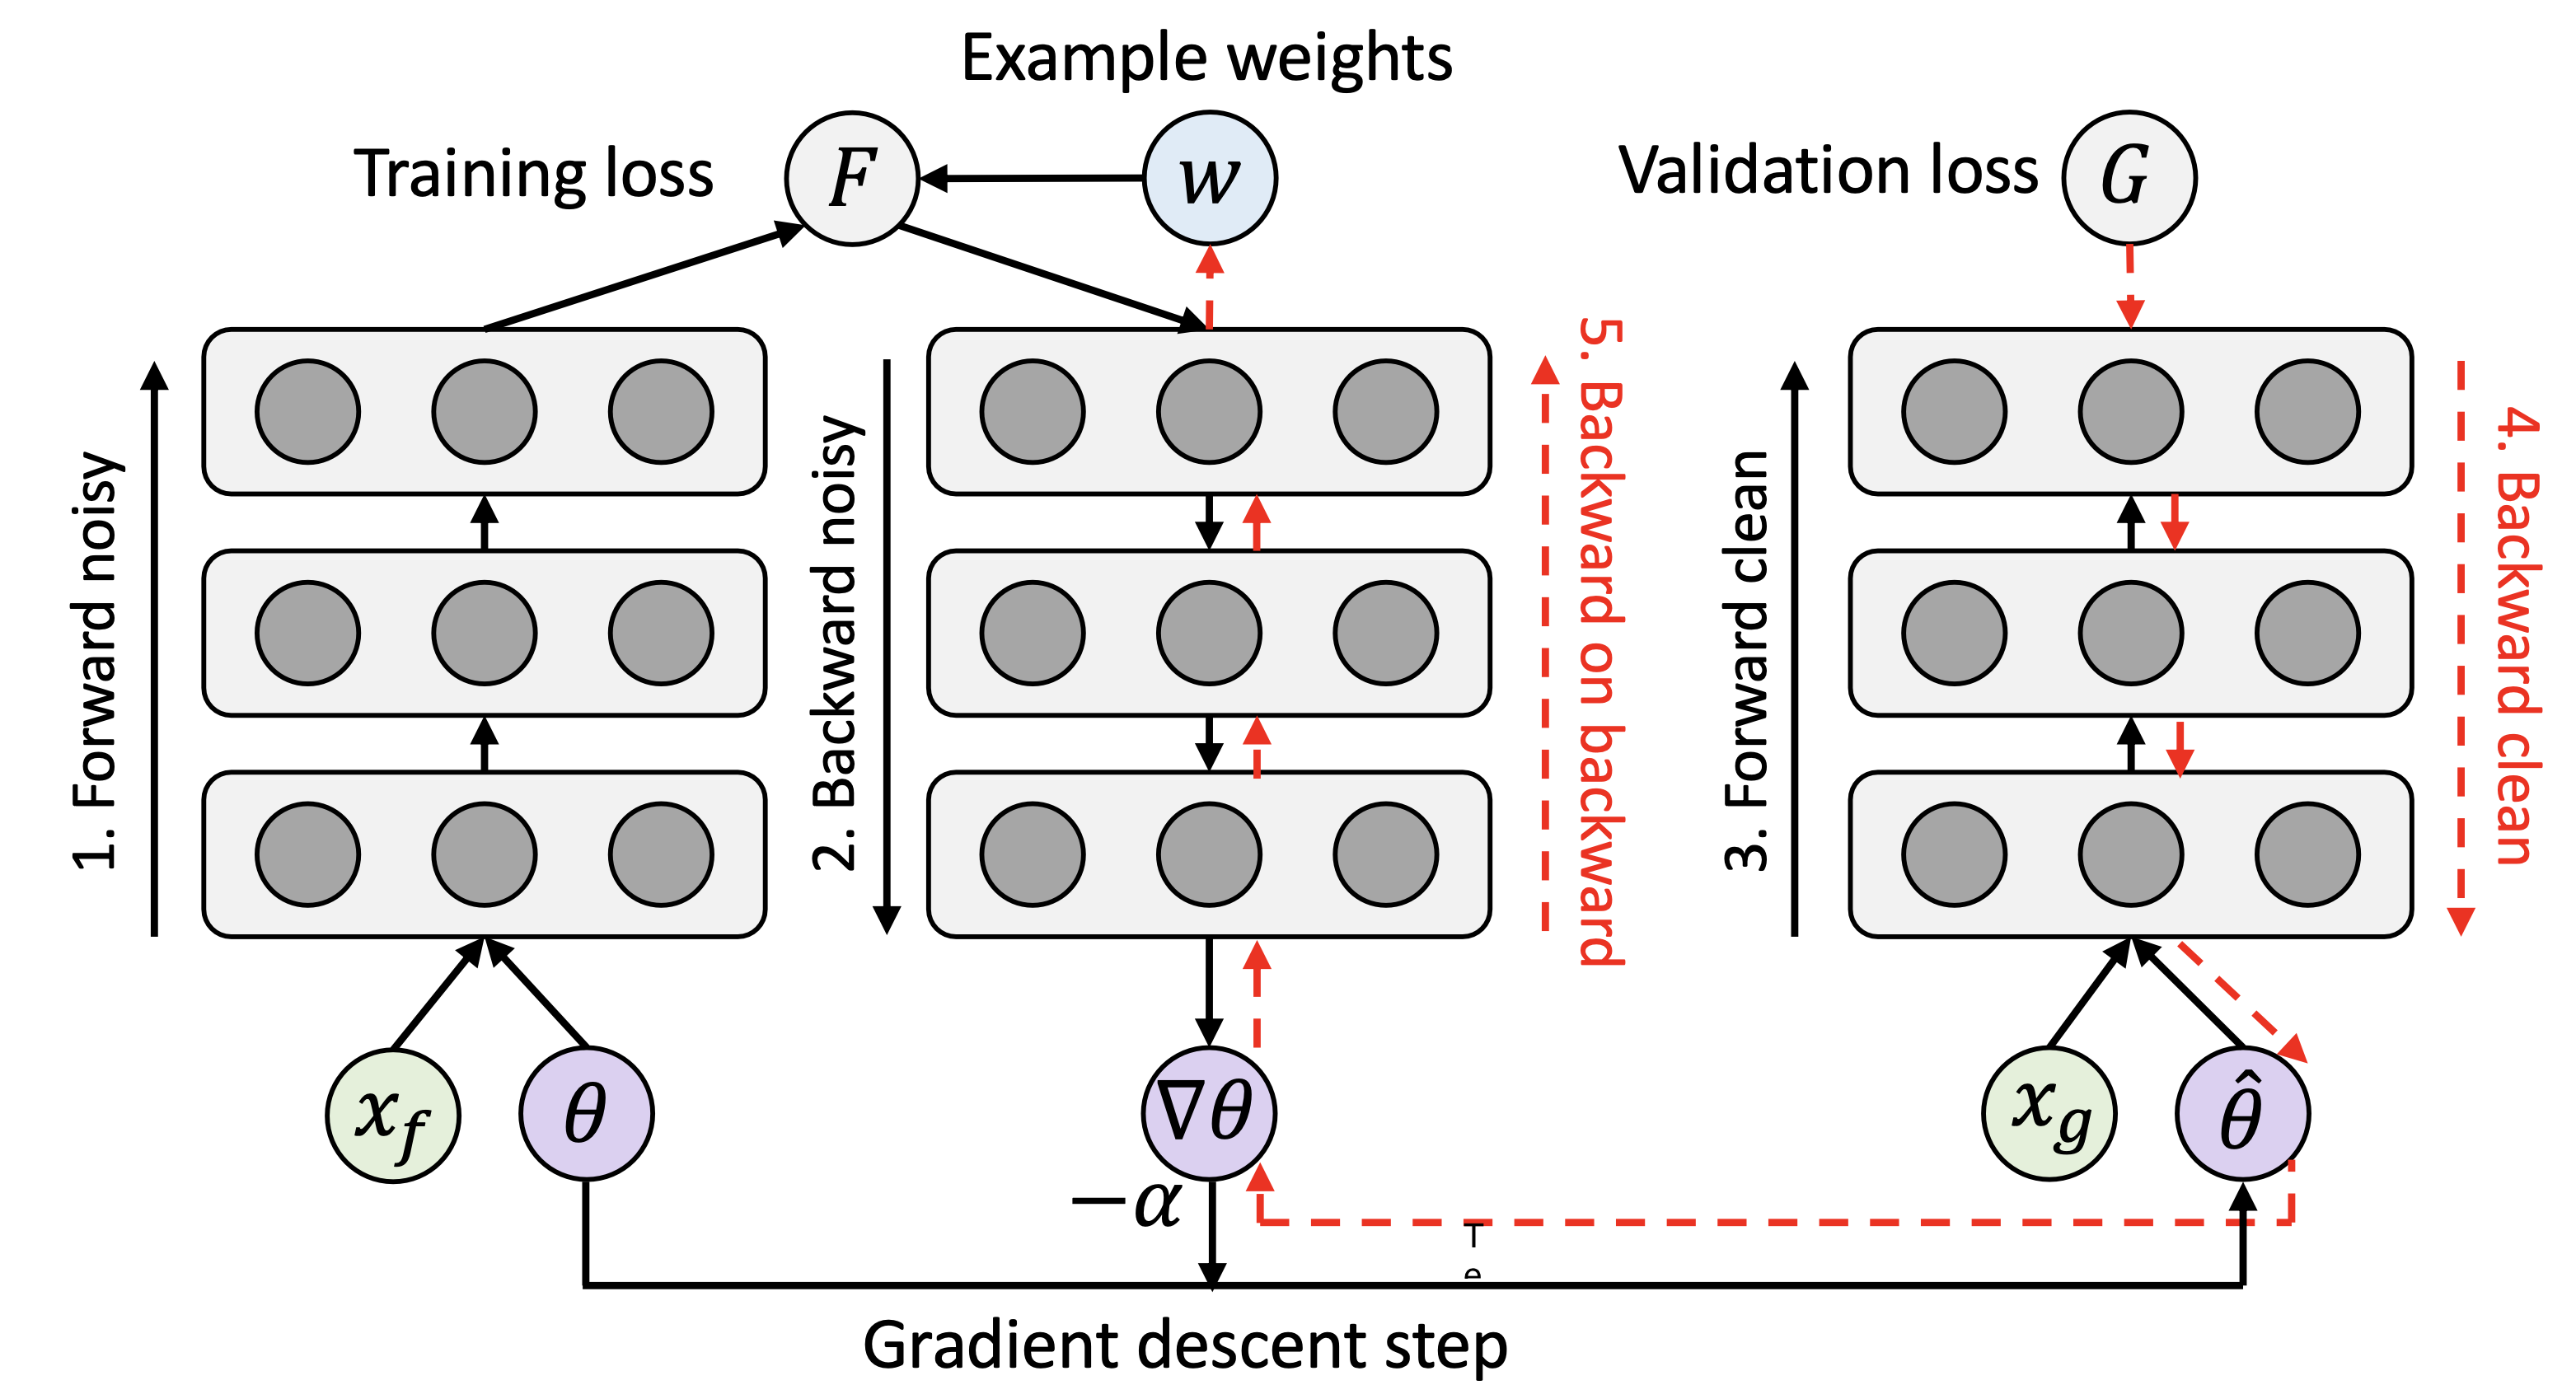
\includegraphics[width=6\columnwidth]{figures/comp_graph.png}
\else
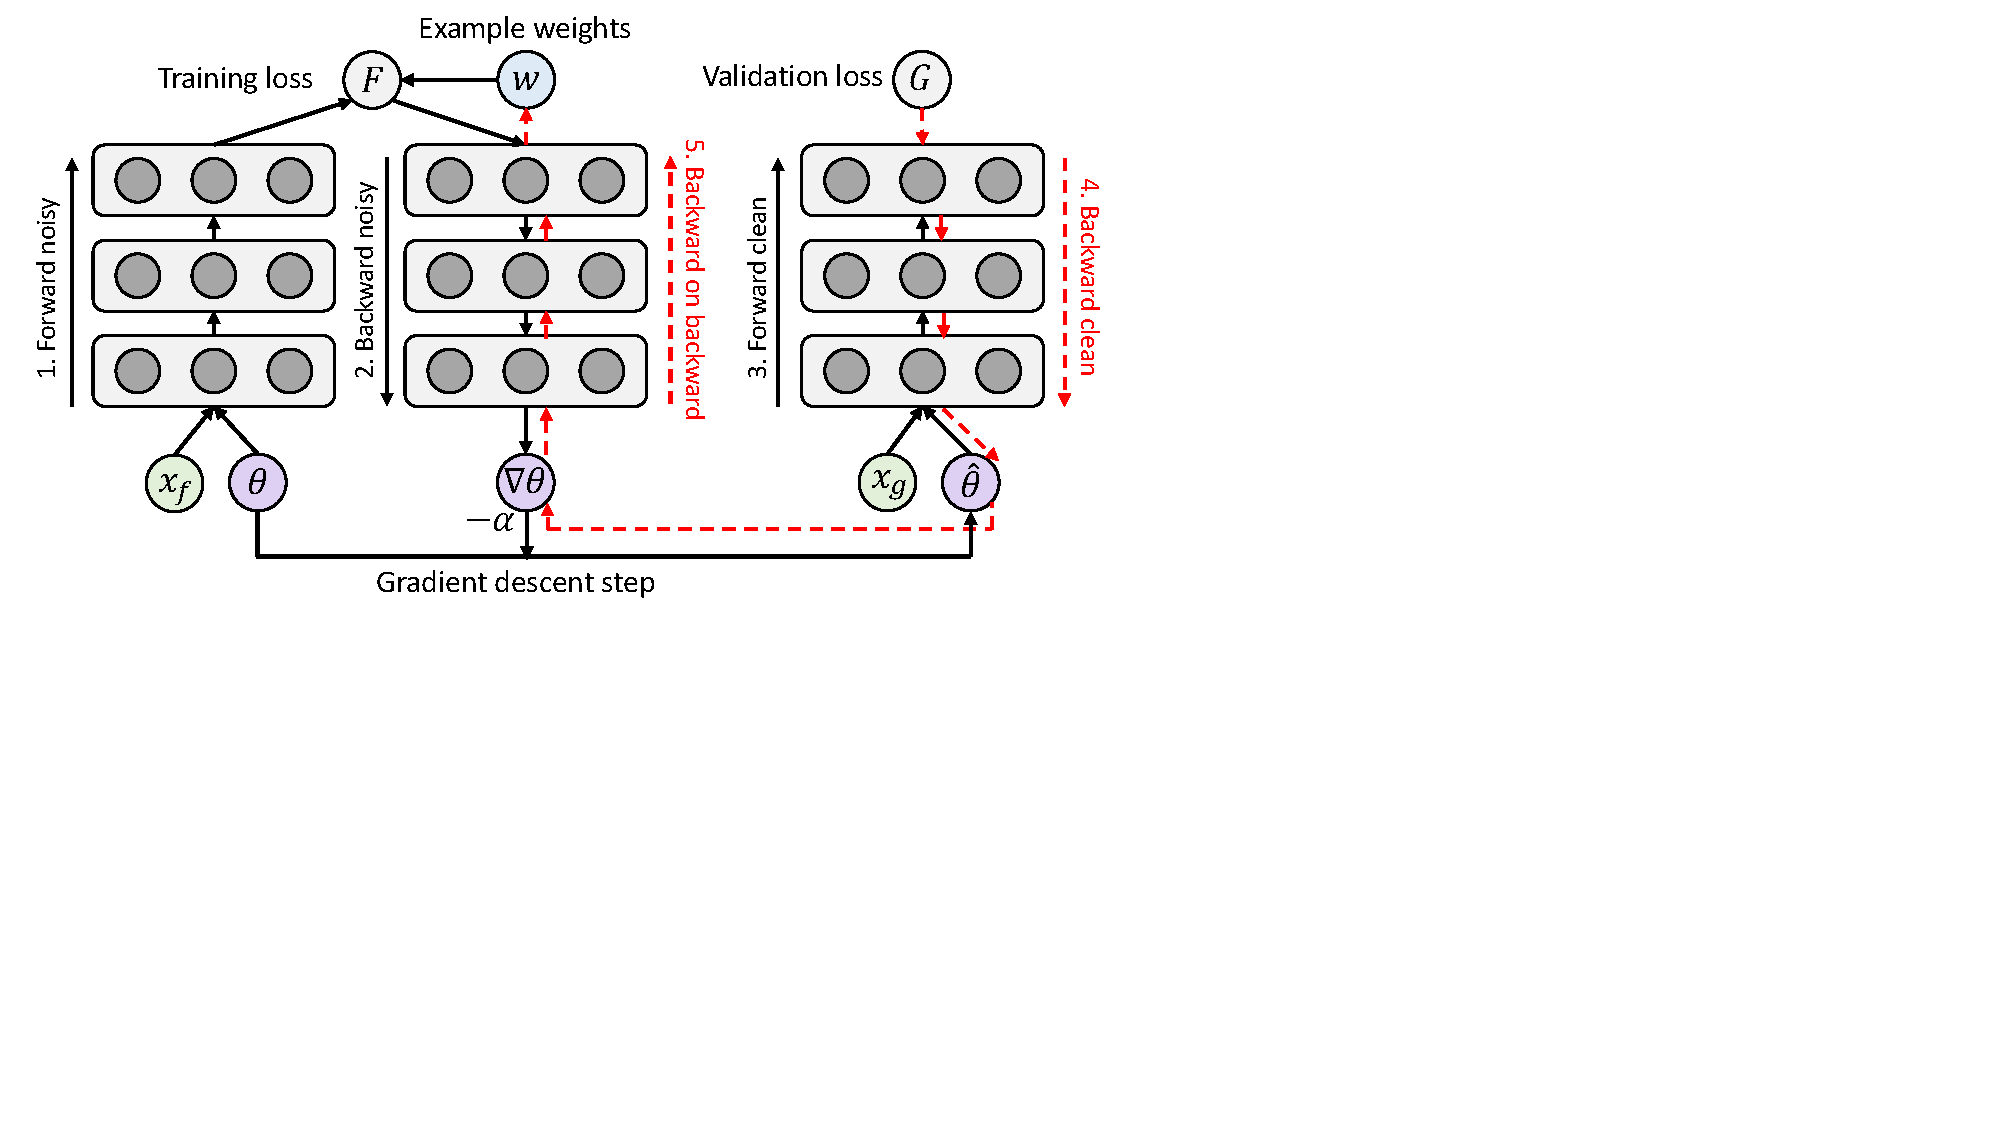
\includegraphics[width=\columnwidth,trim={0cm 8.9cm 15cm 0},clip]{figures/comp_graph.pdf}
\fi
\vspace{-0.1in}
\caption{Computation graph of our algorithm in a deep neural network, which can be efficiently implemented using second order automatic differentiation.}
\label{fig:comp_graph}
\end{figure}
 In an MLP and a CNN, the unnormalized weights can be calculated based on
the sum of the correlations of layerwise activation gradients and input activations. In more general
networks, we can leverage automatic differentiation techniques to compute the gradient of the
validation loss wrt. the example weights of the current batch. As shown in
Figure~\ref{fig:comp_graph}, to get the gradients of the example weights, one needs to first unroll
the gradient graph of the training batch, and then use backward-on-backward automatic
differentiation to take a second order gradient pass (see Step 5 in Figure~\ref{fig:comp_graph}). We
list detailed step-by-step pseudo-code in Algorithm~\ref{alg:ad}. This implementation can be
generalized to any deep learning architectures and can be very easily implemented using popular deep
learning frameworks such as TensorFlow \cite{tensorflow}.

\begin{minipage}{\columnwidth}
\begin{algorithm}[H]
\caption{Learning to Reweight Examples using Automatic Differentiation}
\label{alg:ad}
\begin{algorithmic}[1]
\REQUIRE $\theta_0$, $\mathcal{D}_f$, $\mathcal{D}_g$, $n$, $m$
\ENSURE $\theta_T$
\FOR{$t=0$ ... $T-1$}
\STATE $\{X_f, y_f\} \gets$ \text{SampleMiniBatch}($\mathcal{D}_f$, $n$)
\STATE $\{X_g, y_g\} \gets$ \text{SampleMiniBatch}($\mathcal{D}_g$, $m$)
\STATE $\hat{y}_f \gets \text{Forward}(X_{f}, y_{f}, \theta_t)$
\STATE $\epsilon \gets 0$; $l_f \gets \sum_{i=1}^n \epsilon_i C(y_{f,i}, \hat{y}_{f,i})$
\STATE $\nabla \theta_t \gets \text{BackwardAD}(l_f, \theta_t)$
\STATE $\hat{\theta}_t \gets \theta_t - \alpha \nabla \theta_t$
\STATE $\hat{y}_g \gets \text{Forward}(X_{g}, y_{g}, \hat{\theta}_t)$
\STATE $l_g \gets \frac{1}{m} \sum_{i=1}^m C(y_{g,i}, \hat{y}_{g,i})$
\STATE $\nabla \epsilon \gets \text{BackwardAD}(l_g, \epsilon)$  \label{lst:line:bb}
\STATE $\tilde{w} \gets \max(-\nabla \epsilon, 0)$; $w \gets \frac{\tilde{w}}{\sum_j \tilde{w} + \delta(\sum_j \tilde{w})}$
\STATE $\hat{l}_f \gets \sum_{i=1}^n w_i C(y_i, \hat{y}_{f,i})$
\STATE $\nabla \theta_t \gets \text{BackwardAD}(\hat{l}_f, \theta_t)$
\STATE $\theta_{t+1} \gets \text{OptimizerStep}(\theta_t, \nabla \theta_t)$
\ENDFOR
\end{algorithmic}
\end{algorithm}
\end{minipage}

\paragraph{Training time} Our automatic reweighting method will introduce a constant factor of
overhead. First, it requires two full forward and backward passes of the network on training and
validation respectively, and then another backward on backward pass (Step 5 in
Figure~\ref{fig:comp_graph}), to get the gradients to the example weights, and finally a backward
pass to minimize the reweighted objective. In modern networks, a backward-on-backward pass usually
takes about the same time as a forward pass, and therefore compared to regular training, our method
needs approximately 3$\times$ training time; it is also possible to reduce the batch size of the
validation pass for speedup. We expect that it is worthwhile to spend the extra time to avoid the
irritation of choosing early stopping, finetuning schedules, and other hyperparameters.

\subsection{Analysis: convergence of the reweighted training}
Convergence results of SGD based optimization methods are well-known \cite{svrg}. However it is
still meaningful to establish a convergence result about our method since it involves optimization
of two-level objectives (Eq. \ref{eq:theta_star}, \ref{eq:w_star}) rather than one, and we further
make some first-order approximation by introducing Eq. \ref{eq:meta-gradient}. Here, we show
theoretically that our method converges to the critical point of the validation loss function under
some mild conditions, and we also give its convergence rate. More detailed proofs can be found in
the 
\if\arxiv1
Appendix~\ref{sec:lemproof},~\ref{sec:thmproof}.
\else
Supplementary Materials.
\fi

\begin{deff}\label{deff:lipandbound}
A function $f(x): \mathbb{R}^d \to \mathbb{R}$ is said to be Lipschitz-smooth with constant $L$ if
\begin{align*}
\lVert \nabla f(x) - \nabla f(y) \rVert \leq L \lVert x - y \rVert, \forall x, y \in \mathbb{R}^d.
\end{align*}
\end{deff}
\begin{deff}
$f(x)$ has $\sigma$-bounded gradients if $\lVert \nabla f(x) \rVert \leq \sigma$ for all $x \in
\mathbb{R}^d$.
\end{deff}

In most real-world cases, the high-quality validation set is really small, and thus we could set the
mini-batch size $m$ to be the same as the size of the validation set $M$. Under this condition, the
following lemma shows that our algorithm always converges to a critical point of the validation
loss. However, our method is not equivalent to training a model only on this small validation set.
Because directly training a model on a small validation set will lead to severe overfitting issues.
On the contrary, our method can leverage useful information from a larger training set, and still
converge to an appropriate distribution favored by this clean and balanced validation dataset. This
helps both generalization and robustness to biases in the training set, which will be shown in our
experiments.

\begin{lem}\label{lem:convergence}
% !TEX root = ../main.tex
Suppose the validation loss function is Lipschitz-smooth with constant $L$, and the train loss
function $f_i$ of training data $x_i$ have $\sigma$-bounded gradients. Let the learning rate
$\alpha_t$ satisfies $\alpha_t \leq \frac{2n}{L\sigma^2}$, where $n$ is the training batch size.
Then, following our algorithm, the validation loss always monotonically decreases for any sequence of
training batches, namely,
\begin{align}
\label{eq:converge1}
G(\theta_{t+1}) \leq G(\theta_{t}),
\end{align}
where $G(\theta)$ is the total validation loss
\begin{align}
G(\theta) = \frac{1}{M} \sum_{i=1}^M f^v_i(\theta_{t+1}(\epsilon)).
\end{align}
Furthermore, in expectation, the equality in Eq. \ref{eq:converge1} holds only when the gradient of
validation loss becomes 0 at some time step $t$, namely $\EEsub{G(\theta_{t+1})}{t} = G(\theta_t)$
if and only if $\nabla G(\theta_t) = 0$, where the expectation is taking over possible training
batches at time step $t$.

\end{lem}
Moreover, we can prove the convergence rate of our method to be $O(1/\epsilon^2)$.

\begin{thm}\label{thm:convergencerate}
% !TEX root = ../main.tex
Suppose $G$, $f_i$ and $\alpha_t$ satisfy the aforementioned conditions, then
Algorithm~\ref{alg:ad} achieves $\EE{\lVert \nabla G(\theta_t) \rVert^2} \leq \epsilon$ in
$O(1/\epsilon^2)$ steps. More specifically,
\begin{align}
\min\limits_{0 < t < T} \EE{\lVert \nabla G(\theta_t) \rVert^2} \leq \frac{C}{\sqrt{T}},
\end{align}
where $C$ is some constant independent of the convergence process.

\end{thm}
